\section{Evaluation}
\label{sec:Evaluation}
The graphics and calculations shown in \autoref{sec:Evaluation} were created using the Python libraries Matplotlib \cite{matplotlib}, Scipy \cite{scipy} and Numpy \cite{numpy}.

\subsection{Determination of contrast}
The measured values for the voltages $U_{max}$ and $U_{min}$ for the different polarizer angles $\phi$ are shown in \autoref{tab:contrast}. 
The average value is formed from the 3 measurements and the contrast is thus calculated according to \autoref{eqn:2}.

\begin{table}[h]
  \centering
  \begin{tabular}{c|c|c|c|c|c|c}
  \hline
  $\phi$ & $U_{max1}$ & $U_{min1}$ & $U_{max2}$ & $U_{min2}$ & $U_{max3}$ & $U_{min3}$ \\ \hline
  \hline
  0 & 2.00 & 1.76 & 1.91 & 1.68 & 1.83 & 1.68 \\ \hline
  15 & 1.74 & 0.85 & 1.69 & 0.85 & 1.67 & 0.85 \\ \hline
  30 & 1.43 & 0.45 & 1.56 & 0.33 & 1.44 & 0.34 \\ \hline
  45 & 1.51 & 0.22 & 1.59 & 0.16 & 1.53 & 0.15 \\ \hline
  60 & 1.81 & 0.24 & 1.87 & 0.21 & 1.90 & 0.35 \\ \hline
  75 & 2.38 & 0.73 & 2.39 & 0.57 & 2.46 & 0.74 \\ \hline
  90 & 2.23 & 1.86 & 2.22 & 1.61 & 2.48 & 1.86 \\ \hline
  105 & 3.63 & 1.53 & 3.57 & 1.59 & 3.53 & 1.70 \\ \hline
  120 & 5.27 & 0.62 & 5.31 & 0.54 & 5.24 & 0.86 \\ \hline
  135 & 6.49 & 0.25 & 6.00 & 0.31 & 5.87 & 0.44 \\ \hline
  150 & 5.59 & 0.64 & 5.37 & 0.70 & 5.37 & 0.61 \\ \hline
  165 & 4.02 & 1.41 & 3.61 & 1.37 & 3.83 & 1.33 \\ \hline
  180 & 2.04 & 1.76 & 2.14 & 1.80 & 1.72 & 2.16 \\ \hline
  \end{tabular}
  \caption{Measured voltages for different polarizer angles.}
  \label{tab:contrast}
\end{table}
In \autoref{fig:contrast} the contrast is plotted against the polarizer angle $\phi$. Also the fit of the data points to a sinusoidal function of the form
\begin{equation}
  f(x) = a \cdot \sin(b \cdot x + c)
\end{equation}
is shown.
The fit parameters are
\begin{align*}
  a &= \SI{0.867(0.016)}{}, \\
  b &= \SI{2.022(0.015)}{}, \\
  c &= \SI{-0.127(0.018)}{}.
\end{align*}
The maximum contrast occurs at 135°, where the contrast is $C = \SI{0.897(0.024)}{}$.
\begin{figure}[H]
  \centering
  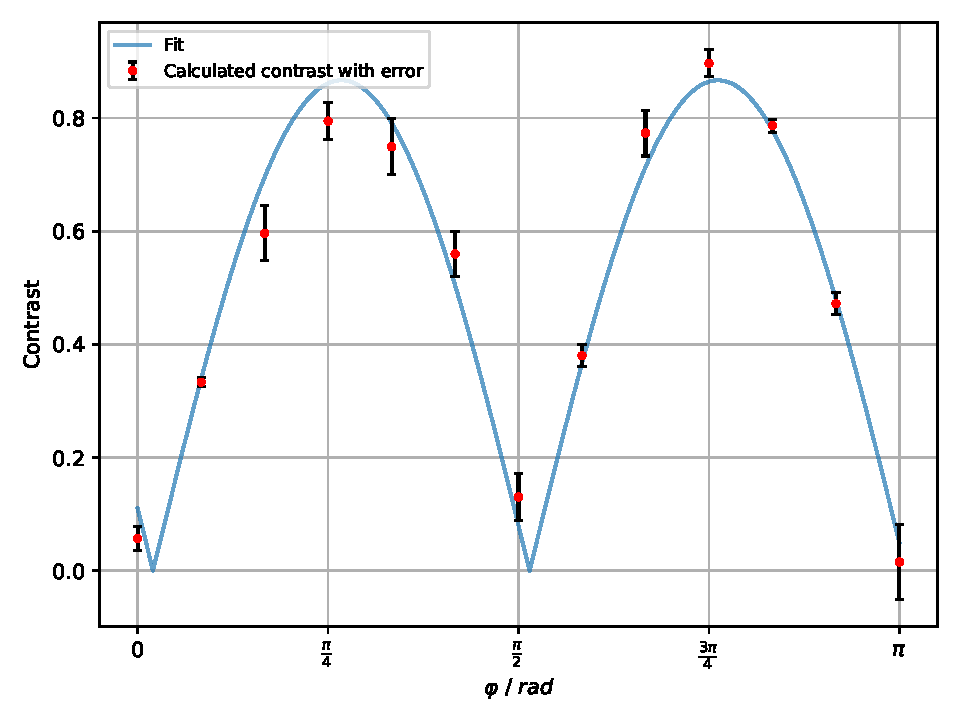
\includegraphics[width=\textwidth]{build/contrast.pdf}
  \caption{Contrast plotted against the polarizer angle $\phi$.}
  \label{fig:contrast}
\end{figure}

\newpage

\subsection{Refractive index of glass}
To determine the refractive index of the glass plate, \autoref{eq:glassn} is used. 
Needed for this calculation are the maxima counts listed in \autoref{tab:refractive_index} and the wavelength of the light source $\lambda = \SI{632.8}{\nano\meter}$.
Furthermore, the thickness of the glass plates is $d = \SI{1}{\milli\meter}$ and the angles are $\theta = \theta_0 = \SI{10}{\degree}$.
\begin{table}[H]
  \centering
  \begin{tabular}{c|c}\hline
    \hline
    counts & counts \\ \hline
    34 & 34 \\ \hline
    30 & 34 \\ \hline
    30 & 33 \\ \hline
    34 & 31 \\ \hline
    34 & 32 \\ \hline
    34 & 32 \\ \hline
  \end{tabular}
  \caption{Maxima counts for the refractive index measurement.}
  \label{tab:refractive_index}
\end{table}
The values are averaged to $M_{mean} = \SI{32.4(1.6)}{}$ and the refractive index is calculated to be $n = \SI{1.51(0.04)}{}$.
\newpage
\subsection{Refractive index of air}
In \autoref{tab:air} the measured values for $p$ and the corresponding maxima counts are shown.
\begin{table}[H]
  \centering
  \begin{tabular}{c|c|c|c|c|c}
  \hline
  $p\,/\,$mBar & count1 & count2 & count3 & count4 & count5 \\ \hline
  \hline
  50 & 3 & 2 & 2 & 3 & 2 \\ \hline
  100 & 6 & 4 & 4 & 4 & 4 \\ \hline
  150 & 8 & 6 & 6 & 6 & 6 \\ \hline
  200 & 10 & 8 & 8 & 8 & 8 \\ \hline
  250 & 12 & 10 & 10 & 10 & 10 \\ \hline
  300 & 14 & 12 & 12 & 12 & 12 \\ \hline
  350 & 16 & 14 & 14 & 14 & 14 \\ \hline
  400 & 18 & 17 & 16 & 16 & 16 \\ \hline
  450 & 20 & 19 & 18 & 18 & 18 \\ \hline
  500 & 22 & 21 & 20 & 20 & 21 \\ \hline
  550 & 25 & 23 & 23 & 23 & 23 \\ \hline
  600 & 27 & 25 & 25 & 25 & 25 \\ \hline
  650 & 29 & 27 & 27 & 27 & 27 \\ \hline
  700 & 32 & 29 & 29 & 29 & 29 \\ \hline
  750 & 34 & 31 & 31 & 31 & 31 \\ \hline
  800 & 36 & 33 & 33 & 33 & 33 \\ \hline
  850 & 38 & 36 & 36 & 36 & 35 \\ \hline
  900 & 44 & 38 & 38 & 38 & 37 \\ \hline
  950 & 46 & 40 & 40 & 40 & 40 \\ \hline
  991 & 48 & 41 & 41 & 41 & 41 \\ \hline
  \end{tabular}
  \caption{Measured maxima counts for different air pressures.}
  \label{tab:air}
\end{table}
The average of the counts is calculated for each row. To determine the refractive index of air
\autoref{eqn:refractive_index_air} is used. The values for the refractive index are plotted against
the corresponding air pressure in \autoref{fig:air}. Also plotted are the fit of the data points to a linear function of the form
\begin{equation}
  f(x) = a \cdot x + b
\end{equation}
and the theory curve according to the Lorentz-Lorenz \autoref{eqn:lorentz_lorenz}.

\begin{figure}[H]
  \centering
  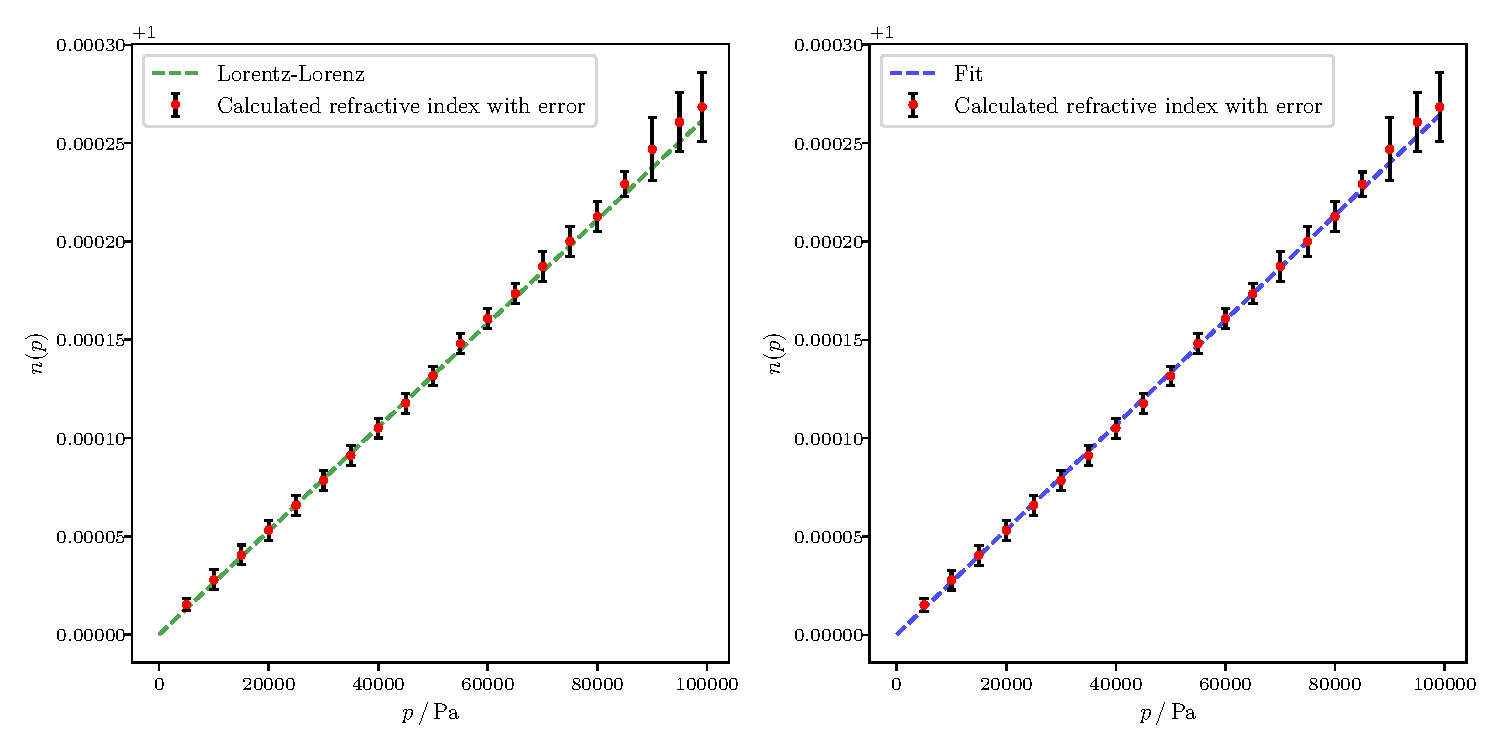
\includegraphics[width=\textwidth]{build/air_and_lorentz.pdf}
  \caption{Refractive index of air plotted against the air pressure, theory curve and fit.}
  \label{fig:air}
\end{figure}

The fit parameters are
\begin{align*}
  a &= \SI{2.66(0.02)e-9}{\per\milli\bar}, \\
  b &= \SI{1.00(0.00)}{}.
\end{align*}
For the Lorentz-Lorenz model following values are used:
\begin{align*}
  A &\approx {0.21\cdot A_{oxygen}+0.79\cdot A_{nitrogen}} \approx \SI{4.2915(0.0024)e-6}{m^3\per\mol},\\
  T &= \SI{293.55(0.1)}{K},\\
  R &= \SI{8.314}{J\per\mol\per K}.
\end{align*}
The values for $A_{oxygen}$\cite{A_oxy} and $A_{nitrogen}$\cite{A_nit} are estimated to be constant.
Now values for the refractive index at normal pressure can be calculated using regression and the Lorentz-Lorenz law.
With $p = \SI{101300}{\pascal}$ and $T = \SI{288.15}{\kelvin}$ the refractive index with the
Lorentz-Lorenz law is $n_{LL} = \SI{1.00027}{}$ and with the regression $n_{reg} = \SI{1.00027}{}$.
\newpage